В 1964 году катастрофическое наводнение потрясло Загреб. Многие здания были полностью 
уничтожены водой, ударившей по их стенам. В этой задаче вам будет дана упрощенная модель города 
перед наводнением, и вы должны будете определить, какие из стен останутся целыми после наводнения. 

Модель состоит из $N$ точек на координатной плоскости и $W$ стен. Каждая стена соединяет пару точек 
и не проходит через другие точки. Модель также удовлетворяет следующим свойствам: 
\begin{itemize}
\item Никакие две стены не пересекаются и не налагаются друг на друга, за исключением того, что они 
могут иметь общие концы; 
\item Каждая стена параллельна либо горизонтальной, либо вертикальной координатной оси. 
\end{itemize}

Изначально вся координатная плоскость суха. В момент времени ноль вода мгновенно затапливает 
внешнее пространство (пространство, не ограниченное стенами). Ровно через час каждая стена, у 
которой с одной стороны "--- вода, а с другой стороны "--- воздух, разрушается под давлением воды. После 
этого вода моментально затапливает пространство, которое перестало быть ограничено целыми стенами. 
В результате этого могут появиться новые стены, у которых с одной стороны вода, а с другой стороны "--- воздух. Еще через час эти стены тоже разрушаются, и вода затапливает новое пространство. Так 
продолжается до тех пор, пока вода не затопит всю территорию. 
Пример процесса разрушения показан на следующем рисунке. 

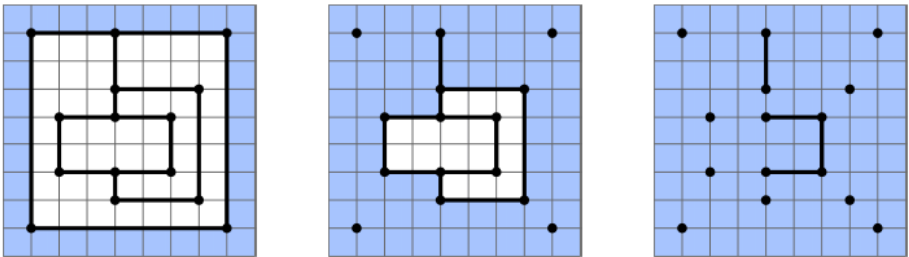
\includegraphics[scale=0.5]{flood.png}

Первая картинка показывает состояние в момент времени 0. Закрашенные клетки соотвествуют затопленной области, а белые --- сухой (воздуху). Вторая картинка показывает состояние через один час. Третья картинка показывет состояние через 2 часа. Вода затопила всю область, и 4 оставшихся стены не могут быть сломаны.


Напишите программу, которая по заданным координатам $N$ точек и описанию $W$ стен, соединяющих 
эти точки, определяет, какие стены останутся целыми после наводнения.
